%% 
%% Copyright 2007-2020 Elsevier Ltd
%% 
%% This file is part of the 'Elsarticle Bundle'.
%% ---------------------------------------------
%% 
%% It may be distributed under the conditions of the LaTeX Project Public
%% License, either version 1.2 of this license or (at your option) any
%% later version.  The latest version of this license is in
%%    http://www.latex-project.org/lppl.txt
%% and version 1.2 or later is part of all distributions of LaTeX
%% version 1999/12/01 or later.
%% 
%% The list of all files belonging to the 'Elsarticle Bundle' is
%% given in the file `manifest.txt'.
%% 
%% Template article for Elsevier's document class `elsarticle'
%% with harvard style bibliographic references

\documentclass[preprint,12pt,authoryear]{elsarticle}

%% Use the option review to obtain double line spacing
%%\documentclass[authoryear,preprint,review,12pt]{elsarticle}

%% Use the options 1p,twocolumn; 3p; 3p,twocolumn; 5p; or 5p,twocolumn
%% for a journal layout:
%% \documentclass[final,1p,times,authoryear]{elsarticle}
%%\documentclass[final,1p,times,twocolumn,authoryear]{elsarticle}
%% \documentclass[final,3p,times,authoryear]{elsarticle}
%% \documentclass[final,3p,times,twocolumn,authoryear]{elsarticle}
%% \documentclass[final,5p,times,authoryear]{elsarticle}
%%\documentclass[final,5p,times,twocolumn,authoryear]{elsarticle}

%% For including figures, graphicx.sty has been loaded in
%% elsarticle.cls. If you prefer to use the old commands
%% please give \usepackage{epsfig}

%% The amssymb package provides various useful mathematical symbols
\usepackage{amssymb}
%% The amsthm package provides extended theorem environments
%% \usepackage{amsthm}

%% The lineno packages adds line numbers. Start line numbering with
%% \begin{linenumbers}, end it with \end{linenumbers}. Or switch it on
%% for the whole article with \linenumbers.
%% \usepackage{lineno}
\usepackage{pgfplotstable,filecontents}
\usepackage{hyperref}
\hypersetup{
    colorlinks=false,
    pdfborder={0 0 0},
}
\usepackage{amsmath}
\usepackage{placeins}  % for \FloatBarrier
\usepackage{svg}
\usepackage{caption}
\usepackage{subcaption}
\usepackage{cancel}
\journal{Ocean Engineering}

\begin{document}

\begin{frontmatter}

    %% Title, authors and addresses

    %% use the tnoteref command within \title for footnotes;
    %% use the tnotetext command for theassociated footnote;
    %% use the fnref command within \author or \affiliation for footnotes;
    %% use the fntext command for theassociated footnote;
    %% use the corref command within \author for corresponding author footnotes;
    %% use the cortext command for theassociated footnote;
    %% use the ead command for the email address,
    %% and the form \ead[url] for the home page:
    %% \title{Title\tnoteref{label1}}
    %% \tnotetext[label1]{}
    %% \author{Name\corref{cor1}\fnref{label2}}
    %% \ead{email address}
    %% \ead[url]{home page}
    %% \fntext[label2]{}
    %% \cortext[cor1]{}
    %% \affiliation{organization={},
    %%            addressline={}, 
    %%            city={},
    %%            postcode={}, 
    %%            state={},
    %%            country={}}
    %% \fntext[label3]{}

    \title{System identification of a physics informed manoeuvring model for better predictions in wind conditions}

    %% use optional labels to link authors explicitly to addresses:
    %% \author[label1,label2]{}
    %% \affiliation[label1]{organization={},
    %%             addressline={},
    %%             city={},
    %%             postcode={},
    %%             state={},
    %%             country={}}
    %%
    %% \affiliation[label2]{organization={},
    %%             addressline={},
    %%             city={},
    %%             postcode={},
    %%             state={},
    %%             country={}}

    \author[1,2]{Martin Alexandersson\corref{cor1}%
        %\fnref{fn1,fn3}
    }
    \ead{maralex@chalmers.se}
    \author[1]{Wengang Mao}
    \author[1]{Jonas W. Ringsberg}
    \author[2]{Martin Kjellberg}


    \affiliation[1]{organization={Dept. of Mechanics and Maritime Sciences, Division of Marine Technology, Chalmers University of Technology},%Department and Organization
        addressline={Hörsalsvägen 7A},
        city={Gothenburg},
        postcode={41296},
        country={Sweden}}


    \affiliation[2]{organization={Research Institutes of Sweden (RISE)},%Department and Organization
        addressline={Chalmers tvärgata 10},
        city={Gothenburg},
        postcode={41296},
        country={Sweden}}

    \cortext[cor1]{Corresponding author}

    \begin{abstract}
        % Move 1 - Background/introduction/situation

System identification offers ways to identify proper models to describe a ship's dynamics in real operational conditions, but also poses some major challenges, such as multicollinearity and generality of the identified model. 
% Move 2 - Present research/purpose
This paper proposes a new physics informed manoeuvring model, where a deterministic semi-empirical rudder model has been added, to guide the identification towards a physically correct model.  
This is an essential building block to solve ship manoeuvring modelling uncertainties from wind, waves, and currents, which are either added for a real sea conditions or important to model for ships with wind-assisted propulsion.
In the physics informed manoeuvring modeling framework, a systematical procedure is developed to establish various force/motion components within the manoeuvring system by the inverse dynamics regression. 
% Move 3 - Methods/materials/subjects/procedures
The novel test case wind powered pure car carrier (WPCC) is used to assess the physical correctness. First, a reference model, assumed to resemble the physically correct kinetics, is established via parameter identification on virtual captive zigzag tests. Then, the model tests are used to build both the physics informed model and the uninformed mathematical Abkowitz model for comparison.


% Move 4 - Results/findings
All of the models predicted the zigzag tests with satisfactory agreement and can thus indeed be considered as being mathematically correct; However, the introduction of a semi-empirical rudder model seems to have guided the identification towards a more physically correct calm water hydrodynamic model, with lower multicollinearity and better generalization. The physics informed model predicted forces and moments that were much more in agreement to the reference model than the Abkowitz model did, and can thus be considered as the more physically correct model. 

% Move 5 - Discussion/conclusion/significance

    \end{abstract}

    %%Graphical abstract
    %\begin{graphicalabstract}
    %    %\includegraphics{grabs}
    %\end{graphicalabstract}
    %
    %%%Research highlights
    %\begin{highlights}
    %    \item Research highlight 1
    %    \item Research highlight 2
    %\end{highlights}

    \begin{keyword}
        %% keywords here, in the form: keyword \sep keyword

        %% PACS codes here, in the form: \PACS code \sep code

        %% MSC codes here, in the form: \MSC code \sep code
        %% or \MSC[2008] code \sep code (2000 is the default)

    \end{keyword}

\end{frontmatter}

%% \linenumbers

%% main text
\section{Introduction}
\label{sec:introduction}
%________________________________________
%CaRS Move I "Establish a territory" (Situation):
% * Important area
% * Introducing and reviewing items of previous  research <--(ToDO)
Ship dynamics prediction models have a wide range of applications within: safety enhancements, route planning and optimization, energy efficiency, automatic berthing and autonomous shipping.
Ship manoeuvring is a sub field of ship dynamics with well established system based models.
Multicollinearity is a well known issue that may lead to parameter drift and poor generalization for models that turns out to be  mathematically correct yet physically incorrect.

A drift angle is needed when the ship is traveling on a straight course in wind -- to counteract the wind forces. This wind state is very rare in calm water manoeuvring tests, where the drift angle is almost exclusively accompanied by yaw rate. It has been shown in this paper that it is very hard to identify a physically correct mathematical model, under those conditions.


\begin{figure}[h!]
  \includegraphics[width=.45\textwidth]{figures/trendinyear.jpg}
  \includegraphics[width=.45\textwidth]{figures/kewords23.png}
  \caption{Publication overview within the field of ship maneuverability system identification}
  \label{fig:pub_overview}
\end{figure}

Modern ships gather vast amounts of kinematic data, including high-precision GPS, accelerometers, and inclinometers, etc. This can be referred to as Internet of Ships (IoS) \citep{liu_internet_2016} as sub group to the internet of things (IoT); Safety enhancements, route planning and optimization, energy efficiency, automatic berthing and autonomous shipping are some of the emerging applications \citep{aslam_internet_2020}.
Predictive modeling can be used for IoS to make predictions about future events or outcomes based on gathered historical data.
Predictive modeling using machine learning (ML) techniques is commonly employed for systems with unknown physics, making ML an adaptable choice for forecasting. However, in cases where prior knowledge of a system's physics and structure is available, such as ship manoeuvring, system identification emerges as a valuable alternative. By leveraging established knowledge, system identification models establish causal relationships between variables, which is an important aspect to enable optimization of the ship operation.
A lot of research has been devoted to describe the ship manoeuvring dynamics with system based manoeuvring simulation models such as: \citet{abkowitz_ship_1964,nomoto_steering_1957,norrbin_theory_1971}, MMG model \citep{yasukawa_introduction_2015}, and others.

\begin{figure}[h!]
  \includegraphics[width=.8\textwidth]{figures/wind_drift_research.png}
  \caption{Recent Publications keyword in 2022 and 2023 on ship maneuverability system identification}
  \label{fig:pub_overview}
\end{figure}

Captive model tests is the classical approach to identify the parameters within these models. However, this approach is not practically applicable for the full scale ships; Instead, computational fluid dynamics (CFD) with either direct simulations or virtual captive tests (VCT) has emerged as an interesting option for the full scale ship predictions \citep{liu_predictions_2018,li_ship_2022}.
The CFD requires a complete understanding of the system; Acquiring such knowledge may be possible for some cases, but it is not practical for the complex environment and nonlinearities of a ship operating at sea \citep{miller_ship_2021};
Wind, waves, and currents, add uncertainty to the modelling in the deep sea; Water depth and the bank effect add uncertainty in coastal areas \citep{nielsen_machine_2022};
Even if the sea is flawlessly modelled, long-term predictions with high accuracy will be exposed to deterministic chaos \citep{lorenz_deterministic_1963}.
Together with the other drawbacks of CFD -- such as high computational costs -- data driven models have become an attractive alternative or complement, with an increased number of publications in the past 10-15 years -- especially within autonomous ships \citep{ahmed_survey_2023}.

Many of these papers have shown that hydrodynamic coefficients can effectively be estimated on simulated data where the exact ''physical'' model is assumed known; However in real cases/applications, the mathematical model is just the simplification of real physics (from VCT, model test, sea trials, or full-scale tests), while the complexity of hydrodynamics involved in vessel maneuvering will greatly challenge the simplified empirical mathematical methods without carefully considering the actual physics inside hydrodynamic coefficients and their interactions.

One of the earlier methods where real data was used was proposed in 1976 by \citet{astrom_identification_1976} to develop a linear manoeuvring model that utilized manually recorded data in 1969 aboard the Atlantic Song freighter with Kalman filter (KF) and maximum likelihood estimation. 
The extended Kalman filter (EKF) can also estimate parameters; This technique was used on a nonlinear Nomoto model by \citet{perera_system_2015} and a 3 degree of freedom model by \citet{shi_identification_2009}. The unscented Kalman filter (UKF), which has been proposed as an improvement to the EKF for handling nonlinear systems, was used in \citet{revestido_herrero_two-step_2012}.
Support vector regression (SVR) has also been investigated by \citet{luo_parameter_2016}, \citet{zhu_parameter_2017}, and \citet{wang_parameter_2021}. 

%
%________________________________________
%CaRS Move II "Establish a niche" (Problem):
% * counter claim?
% * gap?
% * question       <------
% * continuation?
The input variables of the manoeuvring model are often strongly linearly dependent; This multicollinearity is a well known issue in parameter identification that may lead to parameter drift and poor generalization; The parameters are thus mathematically correct but physically incorrect \citep{luo_parameter_2016}. 
Using more informative data or simplifying the model -- when possible -- and thereby reducing the number of parameters, is perhaps the most effective ways to mitigate the multicollinearity.
Some other possible remedies are: the difference method \citep{luo_parameter_2016}, principal component analysis (PCA), and partial least squares regression \citep{jian-chuan_parametric_2015}. 

%________________________________________
%CaRS Move III "Occupy the niche" (Solution/Evaluation):
% * outline purpose?
% * list research questions?
% * announce principal findings?            <--
% * stating the value of present research?
% * article structure?                      <--
Another way to mitigate these difficulties is studied in this paper by introducing a physics informed manoeuvring model, which features a new semi-empirical rudder model based on semi-empirical formulas from the literature;
The objective is to identify models that are not just mathematical correct: but also as physically correct as possible.
To evaluate the physical correctness of identified models, two unique datasets from a wind-powered pure car carrier (WPCC) are employed. Data from VCT at various steady-state drift angles, yaw rates, and rudder angles, establish the physically correct kinetics. System identification is conducted via inverse dynamics \citep{faber_inverse_2018} on a second dataset containing a series of manoeuvring model tests with a free model. The identification is conducted for the physics informed models as well as an Abkowitz mathematical manoeuvring model for comparison. The generalization of the models is studied in an idealized wind state.

For the completeness of this paper; The research methodology is described in \autoref{sec:methodology} -- including the VCT regression, and the inverse dynamics. The physics informed manoeuvring model is introduced in \autoref{sec:ship_models} followed by \autoref{sec:case_study} about the case study ship. Results are presented in \autoref{sec:results}, which are then discussed in \autoref{sec:discussion}. The conclusions of this research are presented in \autoref{sec:conclusions}.

% Old version:
%Prediction of ship maneuverability, which relies on accurate mathematical models to simulate, e.g., Turning Circle Maneuver, Zig-zag Maneuver, etc., is essential for both ship design and intelligent ship navigation. The mathematical ship maneuverability models require inputs of hydrodynamic forces and moments acting on the ship hull, commonly known as “hydrodynamic coefficients”, “maneuvering coefficients” or “maneuvering derivatives” in non-dimensional form. Various approaches have been proposed to derive those non-dimensional hydrodynamic coefficients by different parameter identification methods, such as simple regression, SVM, Kalman filter, and inverse dynamics, such as Tongtong et al. (2020), Zou et al. (2022), Alexandersson et al. (2021, 2022, 2023), ... In Tongtong et al. (2021) and Alexandersson et al. (2022), different mathematical models have been investigated to describe the most accurate and robust ship maneuvering simulations, also referred to the system identification methods.

%However, it should be noted that most research activities aimed to identify a ship's maneuverability mathematical models are built on a ship's simulation data, i.e., a type of inverse engineering to find the model used to simulate the ship maneuvering data. While for practical application, the only reliable source of hydrodynamic coefficients is a model test (ABS 2006), which should also be validated later by full scale test /sea trial). Therefore, several knowledge gaps should be investigated to researched to close the gap between purely simulation-based PIM and generic application of the identified MM model from model to actual usage:
%\begin{enumerate}
%    \item the parameter identification method based on the simulation data can effectively estimate the hydrodynamic coefficients since the exact "psychical" mathematical model is assumed known. In real cases/applications, the mathematical model is just the simplification of real physics (from VCT, model test, sea trials, or full-scale tests), while the complexity of hydrodynamics involved in vessel maneuvering will greatly challenging the simplified empirical mathematical methods without carefully considering the actual physics inside hydrodynamic coefficients and their interactions (ABS 2006).
%    \item if some "actual" data (not simulation data) is used to identify the mathematical model, the PIT may be able to give a good prediction of tested maneuvering trajectories, but the identified mathematical maneuverability model may lack of generalization. It means that the model can only be used to predict the ship's maneuverability under the test scenarios, because the mathematical models cannot capture physics in generic maneuvering scenarios.
%    \item to make the method worse, when using non-simulated data for system identification of maneuverability models, the identified model may give wrong physics, i.e., non-physical hydrodynamic forces regressed from the model. Obviously, for this case, the mathematical model identified based on tests from Turning Circle Maneuver can be only reliably used to predict a ship's maneuverability under turning circle tests but not for the zig-zag tests, and vice verse. In some special case, the prediction can be limited to replicating similar test conditions, such as zig-zag tests at certain angles.
%    \item the prediction of ship maneuverability from the mathematical model (established from ideal conditions such as model tests) is required to be validated/verified by "real" environment conditions, such as sea trials or full-scale tests. The drift caused by wind/current that are not considered in the mathematical maneuverability model will cause completely failure of the identified model applied for real prediction cases.
%\end{enumerate}

%Therefore, this study aims to propose a holistic approach to integrate some physical hydrodynamic terms in the mathematical maneuverability model for a more generic ship maneuverability system identification. This approach can make use of test data in ideal conditions to establish a physics-guided mathematical maneuverability model, which can predict a ship's maneuverability under more generic maneuvering scenarios.



%
%
%
\section{Ship models}
\label{sec:ship_models}
Two different modular manoeuvring models are used in this paper; They both have identical prediction models for the hull and propeller forces, but different models for the rudder forces. The Physics informed model has a new deterministic semi-empirical rudder model -- proposed in this paper (see \autoref{sec:semiempirical_rudder_model}). The mathematical model -- referred to as the Abkowitz model -- has a data driven mathematical rudder model. 
Except the changed rudder models, the manoeuvring models are similar to the MMG model \citep{yasukawa_introduction_2015}, with some minor enhancements that are presented in the next section.
\FloatBarrier
\subsection{Models}
\label{sec:models}
The ship's kinematics are expressed at midship 
in the surge $X$, sway $Y$, and yaw $N$ degrees of freedoms (see \autoref{fig:reference_frames}) described by \autoref{eq:X}-\autoref{eq:N}, where $X_D$, $Y_D$, and $N_D$ describe the damping forces and moments. Note that these equations have the added mass coupling terms: $Y_{\dot{r}}$, and $N_{\dot{v}}$ -- which are neglected in the MMG model.
%
\begin{figure}[h]
    \centering
    \includesvg{figures/reference_frames.svg}
    \caption{Reference frames.}
    \label{fig:reference_frames}
\end{figure}
%
\begin{equation}
    \label{eq:X}
    \input{equations/mathematical_model_kinetics.X}
\end{equation}
%
\begin{equation}
    \label{eq:Y}
    \input{equations/mathematical_model_kinetics.Y}
\end{equation}
%
\begin{equation}
    \label{eq:N}
    \input{equations/mathematical_model_kinetics.N}
\end{equation}

The damping forces and moments are expressed in a modular way as seen in \autoref{eq:X_D} to \autoref{eq:N_D} and \autoref{fig:force_model},
% Components:
\begin{equation}
    \label{eq:X_D}
    \input{equations/mathematical_model_kinetics.X_D}
\end{equation}
%
\begin{equation}
    \label{eq:Y_D}
    \input{equations/mathematical_model_kinetics.Y_D}
\end{equation}
%
\begin{equation}
    \label{eq:N_D}
    \input{equations/mathematical_model_kinetics.N_D}
\end{equation}
%
\begin{figure}[h]
    \centering
    \includesvg[width=4cm]{figures/force_model.svg}
    \caption{The modular force components.}
    \label{fig:force_model}
\end{figure}
%
where the subscripts: H, P, R, and RHI represent contributions from: hull, propellers, rudders, and rudder hull interaction. Rudder hull interaction having its own element is a difference to the MMG model, where RHI is included in the hull forces.
% Hull:

The hull forces are expressed with the same polynomials as the MMG model, except that the ${X_{vvvv}}'$ coefficient has been omitted and an additional resistance term ${X_u}'$ has been added -- to allow for a more nonlinear resistance (see \autoref{sec:hull}). The nonlinear resistance is possible due to the use of perturbed velocity (see \autoref{sec:prime_system}).

%Propellers:
The total twin screw propeller forces are expressed as,
\begin{equation}
    \label{eq:X_P}
    \input{equations/mathematical_model_kinetics.X_P}
\end{equation}
%
\begin{equation}
    \label{eq:Y_P}
    \input{equations/mathematical_model_kinetics.Y_P}
\end{equation}
%
\begin{equation}
    \label{eq:N_P}
    \input{equations/mathematical_model_kinetics.N_P}
\end{equation}
The surge forces from the propellers are calculated as the propeller thrust times a thrust deduction coefficient $X_{thrust}=(1-t)$ as shown in \autoref{eq:X_P_port} and a small yawing moment contribution as seen in \autoref{eq:N_P_port}, where $y_{pport}$ is the propellers transverse coordinate. The thrusts from the propellers $T_{port},T_{stbd}$ are taken from the the model tests measurements, and VCT calculations, since modelling of propeller forces is not of primary focus in this paper.
\begin{equation}
    \label{eq:X_P_port}
    \input{equations/mathematical_model_kinetics.X_P_port}
\end{equation}
\begin{equation}
    \label{eq:N_P_port}
    \input{equations/mathematical_model_kinetics.N_P_port}
\end{equation}

%Rudder hull interaction:
There is an interaction effect between the rudder and hull; The flow in the ship's aft is influenced by the rudder -- which generates lift on the hull surface; Forces from rudder actions are thus generated both on the rudder and on the hull. This effect is modelled by the coefficients $\alpha_H$ and $x_H$ as seen in \autoref{eq:Y_RHI} and \autoref{eq:N_RHI}. This is a changed formulation to the MMG model -- to simplify for regression.
\begin{equation}
    \label{eq:Y_RHI}
    \input{equations/mathematical_model_kinetics.Y_RHI}
\end{equation}
%
\begin{equation}
    \label{eq:N_RHI}
    \input{equations/mathematical_model_kinetics.N_RHI}
\end{equation}

The mathematical rudder model (\autoref{sec:mathematical_rudder_model}) is expressed as a truncated third order Taylor expansion, similar to \citet{abkowitz_ship_1964}. 
The semi-empirical rudder is a new compilation of existing semi-empirical formulas from the literature, which is presented in the next section.

%
\subsection{Semi-empirical rudder model}
\label{sec:semiempirical_rudder_model}
The semi-empirical rudder model is a lifting line model. The surge and sway force are expressed as: rudder lift $L_R$, and rudder drag $D_R$, which are projected on the ship through the rudder inflow angle $\alpha_f$ (see \autoref{eq:X_R_semiempirical} and \autoref{eq:Y_R_semiempirical}).
This angle is a sum of the initial inflow to the rudder at a straight course $\gamma_0$ and the inflow to the rudder $\gamma$ due to: propeller induced speed, drift angle, and yaw rate of the ship; as seen in \autoref{eq:gamma_semiempirical}.
%
\begin{figure}[h]
    \centering
    \includesvg{figures/rudder_flow.svg}
    \caption{Inflow to rudder.}
    \label{fig:reference_frames}
\end{figure}
%
\begin{equation}
    \label{eq:X_R_semiempirical}
    \input{equations/mathematical_model_kinetics.X_R_semiempirical}
\end{equation}
%
\begin{equation}
    \label{eq:Y_R_semiempirical}
    \input{equations/mathematical_model_kinetics.Y_R_semiempirical}
\end{equation}
%
\begin{equation}
    \label{eq:alpha_f_semiempirical}
    \input{equations/mathematical_model_kinetics.alpha_f_semiempirical}
\end{equation}
%
\begin{equation}
    \label{eq:gamma_semiempirical}
    \input{equations/mathematical_model_kinetics.gamma_semiempirical}
\end{equation}
The transverse velocity at the rudder $V_{Ry}$ is calculated with the ship's yaw rate $r$ and the transverse velocity $v$ multiplied by their flow straightening $\kappa_{rtot}$ and $\kappa_{vtot}$ (\autoref{eq:V_R_y_semiempirical}). The flow straightening has a nonlinear dependency of the geometric inflow angle $\gamma_g$ (\autoref{eq:gamma_g_semiempirical}) as seen in \autoref{eq:kappa_r_tot_semiempirical} and \autoref{eq:kappa_v_tot_semiempirical}, so that the flow straightening may vary for different inflow angles, which is an enhancement compared to the MMG model.
The axial velocity at the rudder $V_{RxC}$, including the velocity of the propeller race, is presented in \autoref{sec:velocity_in_the_propeller_slip_stream}.
\begin{equation}
    \label{eq:V_R_y_semiempirical}
    \input{equations/mathematical_model_kinetics.V_R_y_semiempirical}
\end{equation}
%
\begin{equation}
    \label{eq:kappa_r_tot_semiempirical}
    \input{equations/mathematical_model_kinetics.kappa_r_tot_semiempirical}
\end{equation}
%
\begin{equation}
    \label{eq:kappa_v_tot_semiempirical}
    \input{equations/mathematical_model_kinetics.kappa_v_tot_semiempirical}
\end{equation}
%
\begin{equation}
    \label{eq:gamma_g_semiempirical}
    \input{equations/mathematical_model_kinetics.gamma_g_semiempirical}
\end{equation}
The yawing moment is modelled as the sway force times a lever arm $x_R$ as seen in \autoref{eq:N_R_semiempirical}.
\begin{equation}
    \label{eq:N_R_semiempirical}
    \input{equations/mathematical_model_kinetics.N_R_semiempirical}
\end{equation}
%
%
\subsubsection{Rudder lift}
\label{sec:rudder lift}
With inspiration from the work of \citet{villa_numerical_2020}, the total rudder lift is calculated as the sum of the lift from the part of the rudder that is covered by the propeller $L_{RC}$ and the uncovered part $L_{RU}$ as seen in \autoref{eq:L_R_semiempirical} and \autoref{fig:rudder_coverage}.
\begin{equation}
    \label{eq:L_R_semiempirical}
    \input{equations/mathematical_model_kinetics.L_R_semiempirical}
\end{equation}
%
\begin{figure}[h]
    \centering
    \includesvg{figures/rudder_coverage.svg}
    \caption{Rudder areas covered and uncovered by the propeller.}
    \label{fig:rudder_coverage}
\end{figure}
%
The lift forces are calculated with the lift coefficient $C_L$ as seen in \autoref{eq:L_R_U_semiempirical} and \autoref{eq:L_R_C_semiempirical}. These equations are essentially the same except that the lift by the covered part $L_{RC}$ is diminished by the factor $\lambda_R$ (\autoref{eq:lambda_R_semiempirical}) due to the limited radius of the propeller slipstream in the lateral direction \citep{brix_manoeuvring_1993}. A tuning coefficient $C_{Ltune}$ has also been added to these equations.
\begin{equation}
    \label{eq:L_R_U_semiempirical}
    L_{R U } = \frac{A_{R U} C_{L } C_{L tune} V_{R U }^{2} \rho}{2}
\end{equation}
%
\begin{equation}
    \label{eq:L_R_C_semiempirical}
    L_{R C } = \frac{A_{R C} C_{L } C_{L tune} V_{R C }^{2} \lambda_{R } \rho}{2}
\end{equation}
The velocities of the uncovered $V_{RU}$ and covered $V_{RC}$ parts of the rudder are calculated according to \ref{sec:velocity_outside_the_propeller_slip_stream}, and \ref{sec:velocity_in_the_propeller_slip_stream}.

For a none stalling rudder, the lift coefficient $C_L$ is calculated with \autoref{eq:C_L_semiempirical},
\begin{equation}
    \label{eq:C_L_semiempirical}
    C_{L } = \lambda_{gap } \left(\alpha_{} \frac{\partial C_L}{\partial \alpha} + \frac{C_{DC} \alpha_{} \left|{\alpha_{}}\right|}{AR_{e }}\right)
\end{equation}
%
\begin{equation}
    \label{eq:alpha_semiempirical}
    \input{equations/mathematical_model_kinetics.alpha_semiempirical}
\end{equation}
The effective aspect ratio $AR_e$ accounts for the mirror image effect when the rudder is flush with the hull, where the effective aspect ratio is typically assumed to be twice the geometric aspect ratio $AR_g$ (\autoref{eq:AR_e_semiempirical}) \citep{hughes_tempest_2011}.
The WPCC rudder is however not flush to the hull, so that a gap is created between the rudder and rudder horn for larger rudder angles. This gap reduces the pressure difference between the high and low pressure sides in the upper part of the rudder. \citet{matusiak_dynamics_2021} proposed that the gap effect can be modelled as a reduced aspect ratio. Instead a simpler approach is proposed in the this paper -- based on experience. A factor $\lambda_{gap}$ is introduced, which is calculated according to \autoref{eq:lambda_gap_semiempirical}. The gap effect is only activated above a threshold rudder angle $\delta_{lim}$, and the strength of the gap effect is modelled by a factor $s$ as seen in \autoref{fig:gap}.
\begin{equation}
    \label{eq:lambda_gap_semiempirical}
    \input{equations/mathematical_model_kinetics.lambda_gap_semiempirical}
\end{equation}
\begin{figure}[h]
    \centering
    \includesvg[width=0.5\columnwidth]{figures/gap_effect.gap.svg}
    \caption{The rudder lift is reduced by the gap between rudder and rudder horn for larger rudder angles.}
    \label{fig:gap}
\end{figure}
The lift slope of the rudder $\frac{\partial C_L}{\partial \alpha}$ is calculated with \autoref{eq:dC_L_dalpha_semiempirical} where $a_0$ is the section lift curve slope (\autoref{eq:a_0_semiempirical}) and $\Omega$ is the sweep angle of the quarter chord line \citep{lewis_principles_1989}.
\begin{equation}
    \label{eq:dC_L_dalpha_semiempirical}
    \input{equations/mathematical_model_kinetics.dC_L_dalpha_semiempirical}
\end{equation}
%
\begin{equation}
    \label{eq:AR_e_semiempirical}
    \input{equations/mathematical_model_kinetics.AR_e_semiempirical}
\end{equation}
%
\begin{equation}
    \label{eq:AR_g_semiempirical}
    \input{equations/mathematical_model_kinetics.AR_g_semiempirical}
\end{equation}
%
\begin{equation}
    \label{eq:a_0_semiempirical}
    \input{equations/mathematical_model_kinetics.a_0_semiempirical}
\end{equation}
There is also a small nonlinear part to $C_L$ modelled by the cross flow drag coefficient $C_{DC}$ which is calculated for a rudder with squared tip using \autoref{eq:C_D_crossflow_semiempirical} where the taper ratio $\lambda$ is defined as the ratio between the chords at the tip and the root of the rudder (\autoref{eq:lambda__semiempirical}) \citep{hughes_tempest_2011}. 
\begin{equation}
    \label{eq:C_D_crossflow_semiempirical}
    \input{equations/mathematical_model_kinetics.C_D_crossflow_semiempirical}
\end{equation}
%
\begin{equation}
    \label{eq:lambda__semiempirical}
    \input{equations/mathematical_model_kinetics.lambda__semiempirical}
\end{equation}
%
%
\subsubsection{Rudder drag}
\label{sec:rudder_drag}
The total rudder drag $D_R$ is calculated as a sum of the contributions from the parts covered and uncovered by the propeller as seen in \autoref{eq:D_R_semiempirical}.
\begin{equation}
    \label{eq:D_R_semiempirical}
    \input{equations/mathematical_model_kinetics.D_R_semiempirical}
\end{equation}
The drag coefficients: $C_{DC}$, and $C_{DU}$ are calculated with semi-empirical formulas according to \autoref{sec:CD}.



%
%
%
\section{Methodology}
\label{sec:methodology}
The objective of this paper is to investigate the physical correctness of the Abkowitz model and the Physics informed model when the parameters are identified by inverse dynamics regression (ID regression, \autoref{sec:inverse_dynamics}) on a set of calm water zigzag manoeuvres. 
%
The research workflow is summarized in \autoref{fig:methodology}. The workflow consists of two separate sub-processes: on the left hand side the VCT regression (\autoref{sec:VCT_regression}) identifies a Reference model, and on the right hand side the inverse dynamics regression identifies the Abkowitz, and the Physics informed model.
These models are validated by comparison with the Reference model on the model tests and an idealized wind condition.
The Reference model has the Physics informed model structure, but with parameters identified with VCT regression (\autoref{sec:VCT_regression}). 
%The resulting models have been named according to \autoref{tab:model_names}.
The Reference model is assumed to be the more physically correct model, compared to the other two, since it is based on direct CFD calculations of the hydrodynamic forces from a controlled parameter variation.
%
\begin{figure}[h]
    \centering
    \includesvg[width=\columnwidth, pretex=\scriptsize, height=12cm]{figures/methodology2.svg}
    \caption{Research workflow.}
    \label{fig:methodology}
\end{figure}
%
% ToDo: Why 3 methods?
%\begin{table}[h]
%    \caption{Model names are defined by the model structure and regression type.}
%    \label{tab:model_names}
%    \centering
%    \begin{tabular}{l l l}
%        Model name                           & Structure      & Regression \\
%        \hline
%        Reference model & Physics informed & VCT                         \\
%        Physics informede ID  & Physics informed & ID         \\
%        %        Abkowitz VCT & Abkowitz & VCT \\
%        Abkowitz ID                          & Abkowitz       & ID         \\
%    \end{tabular}
%\end{table}
\FloatBarrier
%
\subsection{Prime system}
\label{sec:prime_system}
Variables within some of the equations in this paper are expressed using non dimensional units with the prime system and are then denoted by the prime symbol ($'$). Variables are converted from SI units to the prime system using the denominators in \autoref{tab:prime_system} in \autoref{sec:prime_system_table} for the corresponding physical quantity; where: $U$, and $L$ are the velocity and length between perpendiculars of the ship, and $\rho$ is the water density.
For the calculation of surge velocity $u'$ the perturbed velocity $(u-U_0)$ about a nominal speed $U_0$ is used as seen in \autoref{eq:u_prime}. This is to avoid that $u'$ is 1 for all speeds when the ship is on a straight course (where $u=U$) as in a resistance or self propulsion test. The usage of the perturbed velocity therefore allows for higher order resistance terms in the model such as $X_{u}$, which would otherwise not be possible. 
\begin{equation}
    \label{eq:u_prime}
    u' = \frac{u-U_0}{U}
\end{equation}
In order to have a non dimensional model, $U_0$ is instead expressed as a Froude number within the model (\autoref{eq:Fn0}), where $F_{n0}=0.02$ is used in this paper.
\begin{equation}
    \label{eq:Fn0}
    F_{n0} = \frac{U_0}{\sqrt{g \cdot L}}
\end{equation}

%\subsection{Prime system denominators}
%\label{sec:prime_system_table}
\begin{table}[h]
    \centering
    \caption{Scalings with prime system}
    \label{tab:prime_system}
    \pgfplotstabletypeset[col sep=comma,
        columns={Physical quantity,SI unit,Denominator},
        columns/SI unit/.style={string type},
        columns/Physical quantity/.style={string type},
        columns/Denominator/.style={string type},
        column type=l,	% specify the align method
        every head row/.style={before row=\hline,after row=\hline},	% style the first row
        every last row/.style={after row=\hline},	% style the last row
    ]{tables/prime_system.prime_system.csv"}
\end{table}
\FloatBarrier

\subsection{VCT regression}
\label{sec:VCT_regression}
The parameters within the Reference model are identified by regression on a dataset of virtual captive test (VCT). VCT are computational fluid dynamics (CFD) where the state has been varied according to \autoref{tab:vct_variations}. For instance in the VCT Circle yaw rate $r$ is varied while: surge velocity $u$ is constant, no drift angle ($v=0$), no rudder angle, and the propeller is at the self propulsion point ($\eta_0=1$).

The regression is conducted with ordinary least squares (OLS) multiple linear regression. However, instead of regressing all of the parameters at the same time, the regression is divided into many sub regressions in order to reduce the multicollinearity. The regressions are defined as a step wise process in a regression pipeline. 
The regression pipeline works similarly of solving an equation system; for instance: ${X_{vv}}'$ is determined from the drift angle variation before the circle + drift variation is regressed, so that ${X_{vv}}'$ can be used as a known value when ${X_{vr}}'$ should be determined. The sub regressions must thus be performed in the correct order. 
%The regression pipelines of the Abkowitz model (\autoref{tab:vct_pipeline_abkowitz}), and the Physics informed model (\autoref{tab:vct_pipeline_semiempirical}) are different. 
The regression pipeline of the Physics informed model is shown in \autoref{tab:vct_pipeline_semiempirical}. The semi-empirical rudder is treated as a deterministic model and is therefore not included in the regression. The regression is instead performed on the hull forces $X_H,Y_H,N_H$ obtained from the VCT calculations. The total sway force $Y_D$, and total yawing moment $N_D$ are however used to determine the rudder hull interaction coefficients ${a_H}',{x_H}'$. 
\begin{table}[h!]
    \centering
    \caption{Parameter variations in virtual captive tests where fixed value is indicated by -, varying value by $\sim$ and 0 means that the variable is zero.}
    \label{tab:vct_variations}
    \pgfplotstabletypeset[col sep=comma,
    %columns={Test type,$u$,$v$,$r$,$\delta$,$\eta_0$},
    columns/Test type/.style={string type, column type=l},
    columns/$u$/.style={string type},
    columns/$v$/.style={string type},
    columns/$r$/.style={string type},
    columns/delta/.style={string type},
    columns/$eta_0$/.style={string type},
    %columns/SI unit/.style={string type},
    %columns/Physical quantity/.style={string type},
    %columns/Denominator/.style={string type},
    %column type=l,	% specify the align method
    %every head row/.style={before row=\hline,after row=\hline},	% style the first row
    %every last row/.style={after row=\hline},	% style the last row
    ]{tables/virtual_captive_tests.csv"}
\end{table}
%\begin{table}[h!]
%    \centering
%    \caption{Pipeline for the VCT regression of the Abkowitz model}
%    \label{tab:vct_pipeline_abkowitz}
%    \pgfplotstabletypeset[col sep=comma, string type, column type=l
%    ]{tables/method_VCT_regression.regression_pipeline_abkowitz.csv"}
%\end{table}
\begin{table}[h!]
    \centering
    \caption{Pipeline for the VCT regression of the Physics informed model}
    \label{tab:vct_pipeline_semiempirical}
    \pgfplotstabletypeset[col sep=comma, string type, column type=l
    ]{tables/method_VCT_regression_abkowitz.regression_pipeline_semiempirical.csv"}
\end{table}
\FloatBarrier
%
\subsection{Inverse dynamics and regression}
\label{sec:inverse_dynamics}
Inverse dynamics is a widely used technique within robotics \citep{faber_inverse_2018}; It can be used to estimate the total forces ($X_D,Y_D,N_D$) acting on a ship during motions. The technique can be applied on data from a free model manoeuvring tests or real ship data. The total forces are calculated from the kinematics of the manoeuvring model (\autoref{eq:X} to \autoref{eq:N}). These equations require that the mass, added mass , and the full state of the ship is known -- so that data on the position and orientation of the ship as well as the higher states: velocities, and accelerations, are needed.
However, in the model tests used in this paper, only the position and orientation of the ship model where measured;
The higher states where therefore estimated with an extended Kalman filter (EKF) -- where the manoeuvring model was used as the predictor \citep{alexandersson_wpcc_2022}.

The estimated inverse dynamics forces were regressed with ordinary least squares (OLS) multiple
linear regression to identify the model parameters. The inverse dynamics regression was conducted on zigzag10/10, and zigzag20/20 model test data to port and starboard.  
\FloatBarrier
%
%
%
\section{Case study}
\label{sec:case_study}
The wind powered car carrier (WPCC) has wind assisted ship propulsion (WASP) and can alter between a fully sailing mode, and a fully motoring mode -- and all in between. 
In this paper however, only the motoring mode is considered. Due to the WASP, the WPCC design differs a bit from conventional motoring cargo ship designs; The WPCC has two very large rudders -- the rudders are in fact two to three times as large as they would need to be for a conventional ships. The ship also has fins at the bilge, to generate extra lift while sailing, as seen on the scale model in \autoref{fig:WPCC}. This figure also show two fans, that can be used to simulate wind forces, these were however not used in the manoeuvring tests of this paper.
\begin{figure}[h]
    \centering
    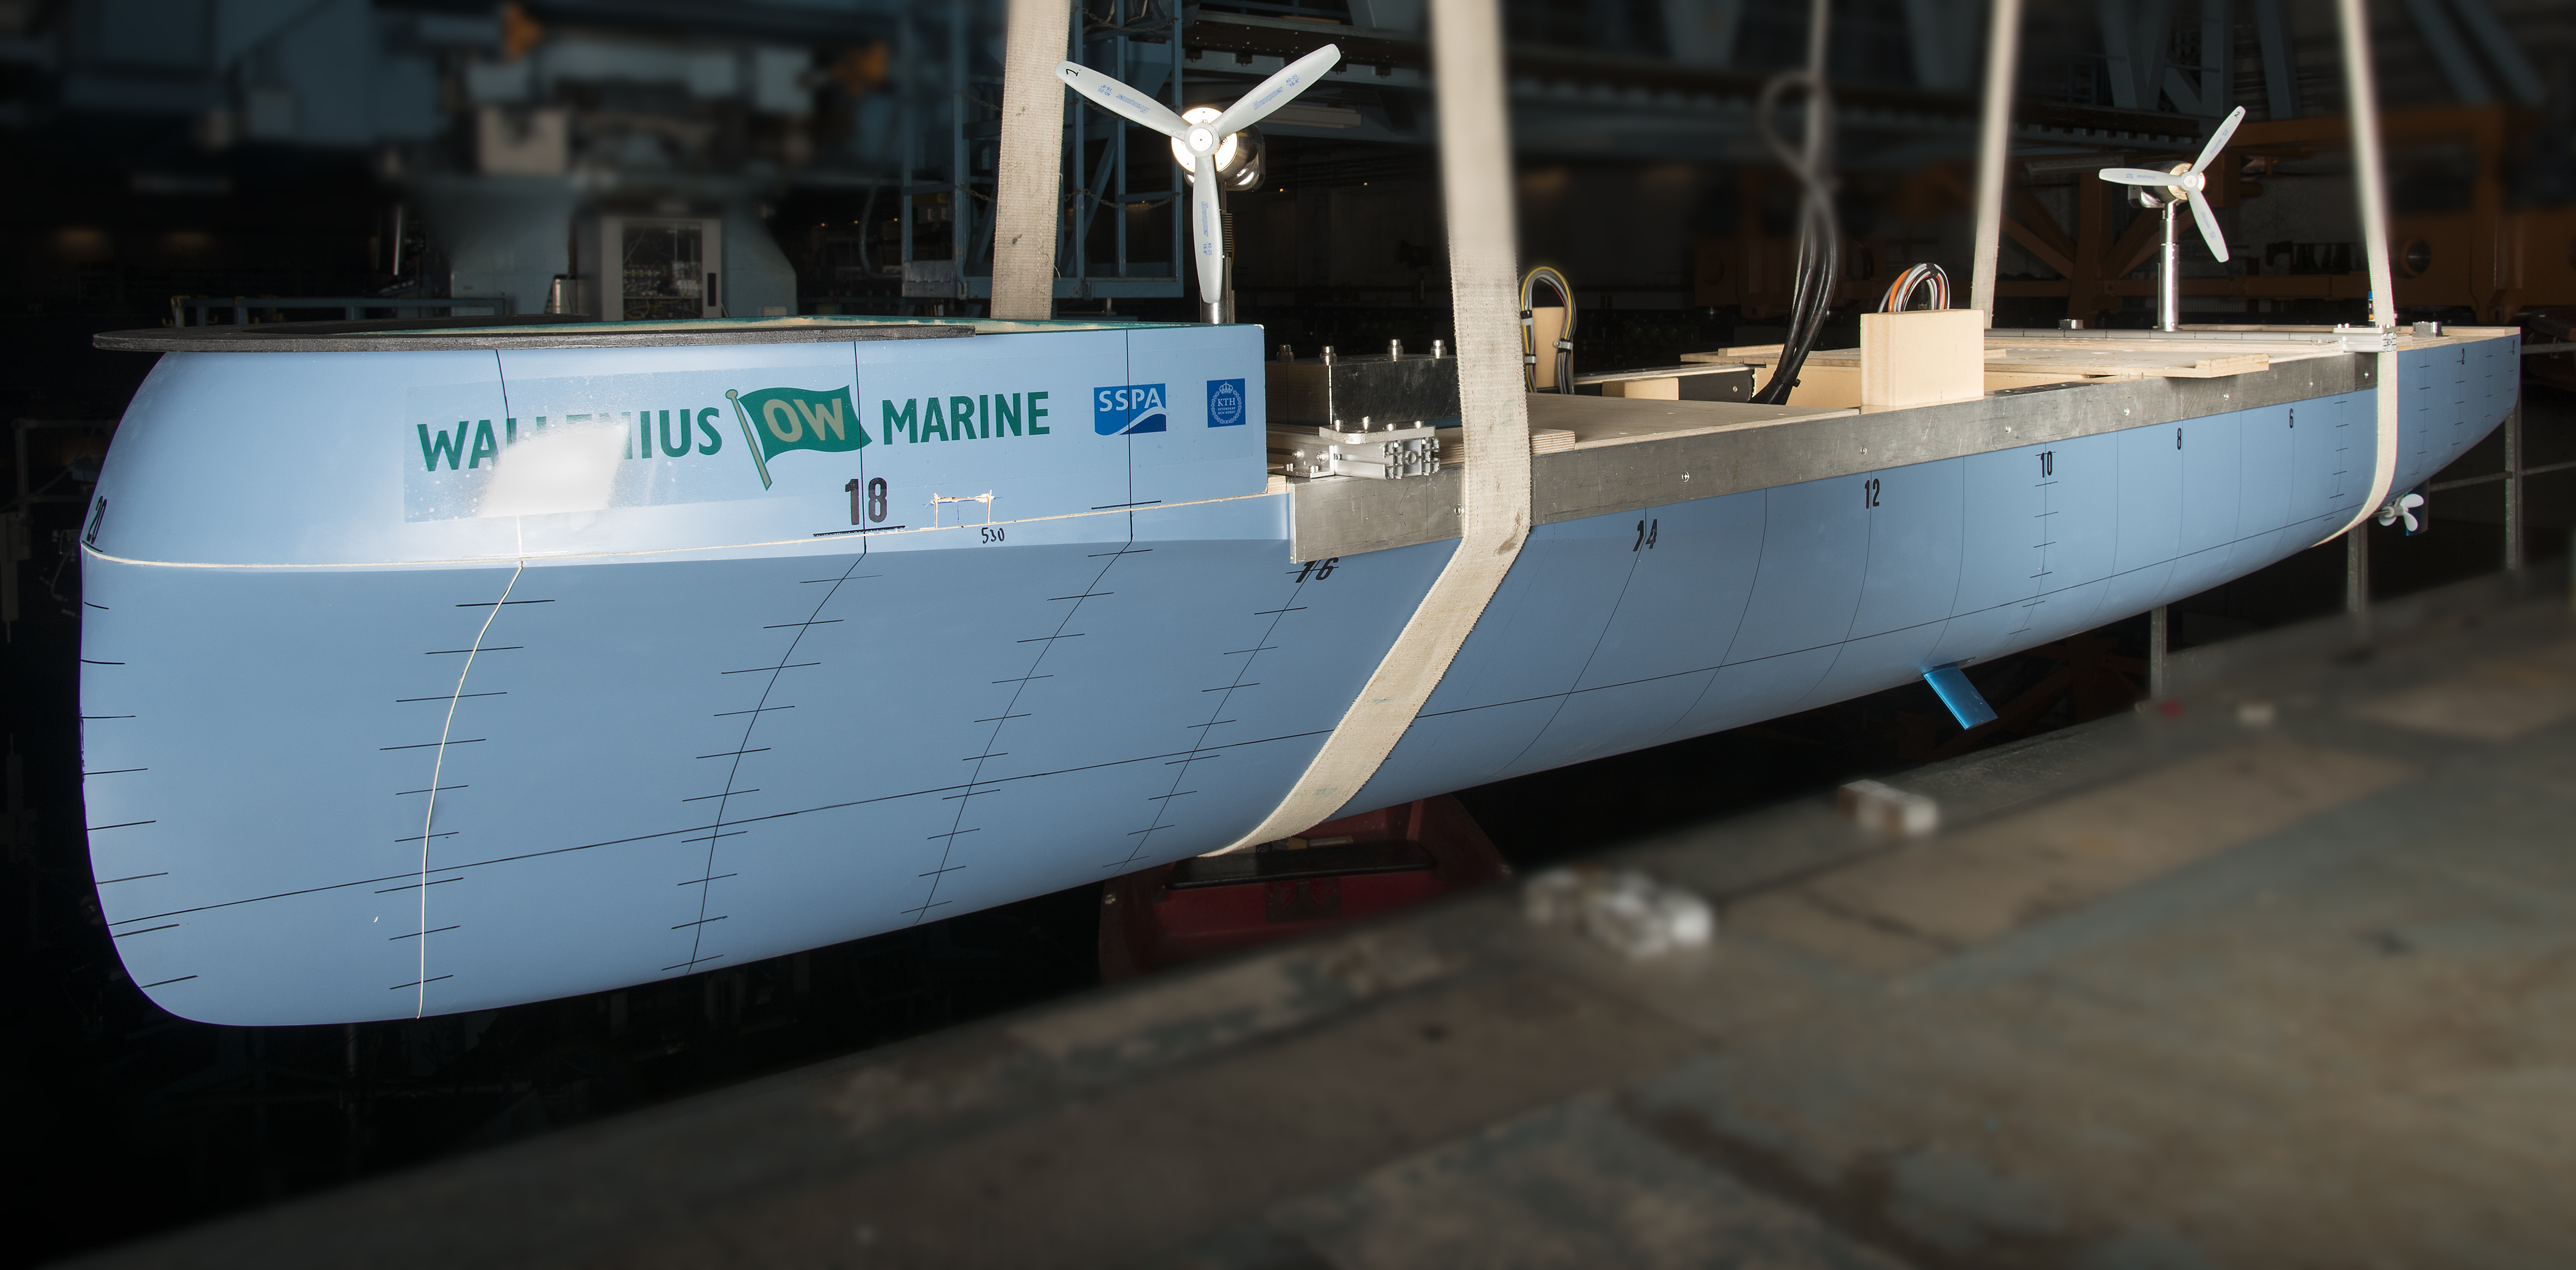
\includegraphics[width=\columnwidth]{figures/5m.jpg}
    \caption{The scale model of the WPCC used in the model tests. Copyright RISE.}
    \label{fig:WPCC}
\end{figure}
\FloatBarrier
\subsection{Parameters}
\label{sec:parameters}
\begin{table}[h]
    \centering
    \caption{Semi-empirical rudder parameters.}
    \label{tab:other_parameters}
    \pgfplotstabletypeset[col sep=comma, column type=r,
    columns/Parameter/.style={column type=c,string type},
    columns/Parameter/.style={column type=c,string type},
    columns/Parameter/.style={column type=c,string type},
    ]{tables/result_models.other_parameters_mcol.csv}
\end{table}
\begin{table}[h]
    \centering
    \caption{Added masses.}
    \label{tab:added_masses}
    \pgfplotstabletypeset[col sep=comma, column type=r,
    columns/Xudot/.style={column name=$X_{\dot{u}}$},
    columns/Yvdot/.style={column name=$Y_{\dot{v}}$},
    columns/Yrdot/.style={column name=$Y_{\dot{r}}$},
    columns/Nvdot/.style={column name=$N_{\dot{v}}$},
    columns/Nrdot/.style={column name=$N_{\dot{r}}$},
    ]{tables/result_models.added_masses.csv}
\end{table}

%
%
%
\section{Results}
\label{sec:results}
The parameters within the models (see \autoref{tab:parameters}) were identified: for the Reference model with VCT regression, for the Abkowitz, and the Physics informed model with inverse dynamics regression (as described in the methodology \autoref{sec:methodology}). 

The parameters used for the semi-empirical rudders are shown in \autoref{tab:other_parameters}. Some manual tuning of the rudder drag was necessary, especially in the neutral rudder case, where the drag was increased almost 8 times as seen for $C_{D0tune}$. The rudder hull interaction coefficient $a_H$ was set to 0.12, so that 12\% of the rudder force is being generated on the ship hull.
\begin{table}[h]
    \centering
    \caption{Identified parameter values.}
    \label{tab:parameters}
    \pgfplotstabletypeset[col sep=comma, column type=r,
    columns/Coefficient/.style={column type=c,string type},
    ]{tables/result_models.parameters.csv}
\end{table}

The validations of these identified models and a closer examination of the identified parameters are presented in this section; The Reference model is compared with the VCT data in \autoref{sec:result_VCT}; All of the models are compared with: the manoeuvring model tests in \autoref{sec:result_MDL}, and with an idealized wind condition in \autoref{sec:wind_state}.
%
\subsection{Predictions of VCT}
\label{sec:result_VCT}
Predictions with the identified Reference model were in good agreement with the corresponding VCT results as seen in \autoref{fig:vct}. The ranges of variations have been chosen to match the states of the model tests, where for instance 10 degrees is the largest drift angle recorded from the zigzag tests (\autoref{fig:vct_drift_angle}). The hull forces are almost linear for these small drift angles and yaw rates; The higher order terms in the hull force model (\autoref{eq:X_H},\autoref{eq:Y_H},\autoref{eq:N_H}) were thus omitted in the VCT, and ID regressions -- to reduce the multicollinearity.
\begin{figure}
     \centering
     \begin{subfigure}[b]{0.49\textwidth}
         \centering
         \includesvg[width=\textwidth]{figures/vct.VCT Drift angle.svg}
         \caption{Drift angles.}
         \label{fig:vct_drift_angle}
     \end{subfigure}
     \hfill
     \begin{subfigure}[b]{0.49\textwidth}
         \centering
         \includesvg[width=\textwidth]{figures/vct.VCT Circle.svg}
         \caption{Yaw rates.}
         \label{fig:vct_circle}
     \end{subfigure}
     %
     \begin{subfigure}[b]{0.49\textwidth}
         \centering
         \includesvg[width=\textwidth]{figures/vct.VCT Rudder angle.svg}
         \caption{Rudder angles.}
         \label{fig:vct_rudder_angle}
     \end{subfigure}
     \hfill
     \begin{subfigure}[b]{0.49\textwidth}
         \centering
         \includesvg[width=\textwidth]{figures/vct.VCT Thrust variation.svg}
         \caption{Thrust variations at 10 degrees rudder angle.}
         \label{fig:vct_thrust_variation}
     \end{subfigure}
     \caption{Forces and moments: total ($D$), hull ($H$), and rudders ($R$), from VCT (lines) and predictions with Reference model (x marks).}
     \label{fig:vct}
\end{figure}
\FloatBarrier
%
\subsection{Predictions of manoeuvring tests}
\label{sec:result_MDL}
Closed loop simulations, with the control logic of the zigzag test, were used to predict the model test experiments. Comparisons of these predictions are shown in \autoref{fig:closed_loop_zigzag10} and \autoref{fig:closed_loop_zigzag20}. The drift angle $\beta$, heading angle $\psi$, and yaw rate $r$, are in good agreement with the experiments for all the models, especially the heading -- which is the most important quantity in zigzag tests; The Abkowitz ID does however have a faster response time.
\begin{figure}[h]
    \centering
    \includesvg[width=\columnwidth]{figures/results.closed_loop_zigzag10.svg}
    \caption{Results from a zigzag10/10 model test compared with closed loop simulations.}
    \label{fig:closed_loop_zigzag10}
\end{figure}
\begin{figure}[h]
    \centering
    \includesvg[width=\columnwidth]{figures/results.closed_loop_zigzag20.svg}
    \caption{Results from a zigzag20/20 model test compared with closed loop simulations.}
    \label{fig:closed_loop_zigzag20}
\end{figure}

An alternative comparison, is to compare model predictions with inverse dynamics forces from the model tests; This comparison gives more detailed information about the forces and moments involved during the manoeuvres. The models predicts the forces and moments for the estimated state of the experiment. Thus, all models predict the same state in contrast to simulations -- where the states may differ as the solutions begin to deviate. Inverse dynamics comparisons are shown in \autoref{fig:ID_zigzag10} for the zigzag10/10, and in \autoref{fig:ID_zigzag20} for the zigzag20/20.    
It seems that the total yawing moments $N_D$ agree well for all models and the experimental data. For the total sway force $Y_R$ the Abkowitz model seem to predict a little bit higher force.  
It can also be seen that the Reference model and Physics informed ID predicts the exact same rudder yawing moment $N_R$, since they both use the same deterministic semi-empirical rudder model -- the yawing moments from the hull $N_H$ are therefore similar for these models. The rudder yawing moment from the Abkowitz ID is however very different; The regression has thus been forced to also make the yawing moments from the hull $N_H$ to be very different -- so that the total yawing moment adds up to be correct. This means that the total yawing moment is the same for all models, but the decomposition of hull and rudder moments turns out to be very different.
\begin{figure}[h]
    \centering
    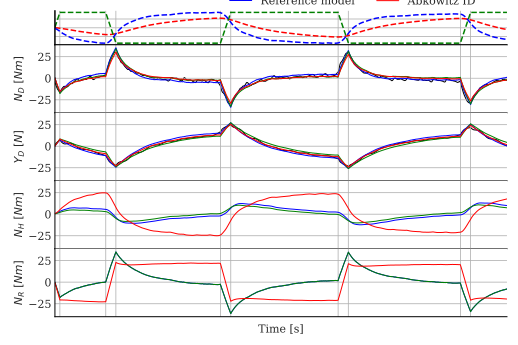
\includegraphics[width=\columnwidth]{figures/results.ID_zigzag10.pdf}
    \caption{Inverse dynamics estimations of $Y_D$, and $N_D$ during a zigzag10/10 model test compared with model predictions.}
    \label{fig:ID_zigzag10}
\end{figure}
\begin{figure}[h]
    \centering
    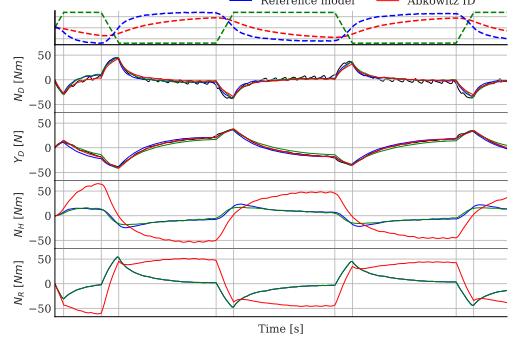
\includegraphics[width=\columnwidth]{figures/results.ID_zigzag20.pdf}
    \caption{Inverse dynamics estimations of $Y_D$, and $N_D$ during a zigzag20/20 model test compared with model predictions.}
    \label{fig:ID_zigzag20}
\end{figure}

The hull force model can be closer examined by decomposing the individual parameter contributions. \autoref{fig:ID_regression_N_decomposition} shows the parameter decomposition for the two models together with the Reference model. The graphs show the joined contributions for parameters related to drift, and yaw rate. It seems that Physics informed ID and the Reference model have very similar parameter decompositions.
The parameter decomposition of the Abkowitz ID is completely different, where almost the entire contribution to the hull yawing moment $N_H$ can be denoted to the yaw rate parameters; The sway force due to drift is also very large.  
\begin{figure}[h]
    \begin{center}
        \includesvg[width=\columnwidth]{figures/results.hull_force_decomposition_zigzag20.svg}
        \caption{Decomposition of hull forces and moments during a zigzag20/20 test for parameters related to drift, yaw rate the prediction models.}
        \label{fig:ID_regression_N_decomposition}
    \end{center}
\end{figure}
Possible implications of that the Abkowitz model have this physically incorrect decomposition of the hull's drift angle and yaw rate dependence will be further investigated in the next section.
\FloatBarrier
%
\subsection{Predictions of an idealized wind state}
\label{sec:idealized_wind_state}
Predictions have been conducted for an idealized wind state, in order to assess the generalization of the  identified models. The idealized wind state is a very simplified hydrodynamic condition where the models have a drift angle, but no yaw rate, or rudder angle; This is meant to represent a state where the ship is experiencing a static drift angle for a long time -- induced by a side wind force.
The prediction results for the idealized wind condition are shown in \autoref{fig:result_wind_state}. The sway force $Y_D$ of the Physics informed model is very similar to the Reference model; For the Abkowitz model the sway force seems to be too large. The yawing moment $N_D$ is under predicted by both models, but the difference is much larger for the Abkowitz model. 
This is because most of the yawing moment is denoted to the yaw rate coefficients (as previously stated in \autoref{sec:result_MDL}) -- which are not activated in the wind state. 
The Physics informed model seems to have a split between the yaw rate and drift angle dependent coefficients that is much more similar to the more physically correct Reference model.
\label{sec:wind_state}
\begin{figure}[h!]
    \includegraphics[width=\columnwidth]{figures/result_wind_state.forces.pdf}
    \caption{Total sway force and yawing moment from the models at various drift angles.}
    \label{fig:result_wind_state}
\end{figure}
\FloatBarrier
%
%\section{Discussion}
%\label{sec:discussion}


%
\section{Conclusions}
\label{sec:conclusions}
\begin{itemize}
    \item A new semi-empirical rudder model has been proposed, combining existing semi-empirical formulas together with some new enhancements: the rudder area covered or uncovered by the propeller slip stream are modelled separately, a new way to model the effect of reduced lift due to gap between rudder and rudder horn has also been proposed.     

    \item All of the identified models in this paper can be considered as mathematically correct, since they all predicted the model tests with satisfactory agreement.
    
    \item The Reference model predicted the VCT with good accuracy and can therefore be considered as the most physically correct model.   
    %
    \item As a logical consequence of this, the mathematical Abkowitz model is considered as physically incorrect, since it predicted very different forces and moments; The regression seems to have made an incorrect decomposition between hull-, and rudder forces, as well as drift angle-, and yaw rate dependent coefficients.  
    %
    \item The physics informed model on the other hand, predicted very similar forces and moments for the model tests and can therefore considered as more physically correct.
    %
    \item Potential problems with the incorrect force decomposition of the Abkowitz model was shown in the lack of generalization of an artificial wind state, where the forces and moments had very large errors. 
    %
    \item The introduction of a semi-empirical rudder model seems to have guided the identification towards a more physically correct model, with lower multicollinearity and better generalization from calm water zigzag tests to wind conditions. 
\end{itemize}
\FloatBarrier
Some points to consider:
\begin{itemize}
    \item Having accurate values for the added masses is very important for the inverse dynamics to deliver forces of the correct magnitude; Especially when a deterministic model such as the semi-empirical rudder is combined with data driven models such as the hull model in this paper. 
    \item The semi-empirical rudder was actually not treated as an entirely deterministic model in this paper; The flow straightening coefficients $\kappa_v$ and $\kappa_r$ where determined from the VCT as well as the rudder hull interaction coefficients $a_H$ and $x_H$. For the time being, some VCT are therefore needed for this model. In the future, when more experience is gained about these coefficients, semi-empirical expressions or rules of thumb can hopefully be developed to make the model fully deterministic.
    \item Persistence of excitation -- the zigzag test is not very informative \citep{sutulo_algorithm_2014}.
    \item For instance Pseudo-Random Binary Sequences (PRBS) \citep{landau_digital_2006} is more informative.
\end{itemize}

%% The Appendices part is started with the command \appendix;
%% appendix sections are then done as normal sections
\appendix
\section{Hull model}
\label{sec:hull}
The hull forces are expressed with the following general polynomials, which are here expressed in prime system units (see \autoref{sec:prime_system}). The parameters that are omitted in this paper are also indicated. 
\begin{equation}
    \label{eq:X_H}
    \input{equations/mathematical_model_kinetics.X_H}
\end{equation}
%
\begin{equation}
    \label{eq:Y_H}
    {Y_H'} = {Y_{0}'} + {Y_{r}'} {r'} + {Y_{v}'} {v'} + {\cancel{Y_{rrr}}'} {r'}^{3} + {\cancel{Y_{vrr}}'} {r'}^{2} {v'} + {\cancel{Y_{vvr}}'} {r'} {v'}^{2} + {\cancel{Y_{vvv}}'} {v'}^{3}
\end{equation}
%
\begin{equation}
    \label{eq:N_H}
    {N_H'} = {N_{0}'} + {N_{r}'} {r'} + {N_{v}'} {v'} + {\cancel{N_{rrr}}'} {r'}^{3} + {\cancel{N_{vrr}}'} {r'}^{2} {v'} + {\cancel{N_{vvr}}'} {r'} {v'}^{2} + {\cancel{N_{vvv}}'} {v'}^{3}
\end{equation}
%
\section{Rudder models}
\label{sec:rudder_models}
\subsection{Mathematical rudder model}
\label{sec:mathematical_rudder_model}
The mathematical rudder model is expressed as a truncated third order Taylor expansion, similar to \citet{abkowitz_ship_1964}, as seen in \autoref{eq:X_R_math} to \autoref{eq:N_R_math}.
\begin{equation}
    \label{eq:X_R_math}
    \input{equations/mathematical_model_kinetics.X_R_math}
\end{equation}
%
\begin{equation}
    \label{eq:Y_R_math}
    \input{equations/mathematical_model_kinetics.Y_R_math}
\end{equation}
%
\begin{equation}
    \label{eq:N_R_math}
    \input{equations/mathematical_model_kinetics.N_R_math}
\end{equation}
\subsection{Semi-empirical rudder model}
\label{sec:semi-empirical_rudder_model}
%\subsubsection{$C_L$}
%\label{sec:CL}
%\input{CL.tex}
\subsubsection{$C_D$}
\label{sec:CD}
The drag coefficients for covered $C_{DC}$ and uncovered $C_{DU}$ are calculated with the similar equations: \autoref{eq:C_D_C_semiempirical}, and \autoref{eq:C_D_U_semiempirical}; where $C_{D0C}$ (\autoref{eq:C_D0_C_semiempirical}) and $C_{D0U}$ (\autoref{eq:C_D0_U_semiempirical}) are the drag at zero rudder angle  and $e_0 = 0.9$ is the Oswald efficiency factor. 
\begin{equation}
    \label{eq:C_D_C_semiempirical}
    \input{equations/mathematical_model_kinetics.C_D_C_semiempirical}
\end{equation}
%
\begin{equation}
    \label{eq:C_D_U_semiempirical}
    \input{equations/mathematical_model_kinetics.C_D_U_semiempirical}
\end{equation}
%
\begin{equation}
    \label{eq:C_D0_C_semiempirical}
    \input{equations/mathematical_model_kinetics.C_D0_C_semiempirical}
\end{equation}
%
\begin{equation}
    \label{eq:C_D0_U_semiempirical}
    \input{equations/mathematical_model_kinetics.C_D0_U_semiempirical}
\end{equation}
$C_{D0C}$ and $C_{D0U}$ will be different due to different Reynolds number $Re$ as seen in \autoref{eq:C_F_C_semiempirical} to \autoref{eq:Re_F_U_semiempirical}.
\begin{equation}
    \label{eq:C_F_C_semiempirical}
    \input{equations/mathematical_model_kinetics.C_F_C_semiempirical}
\end{equation}
%
\begin{equation}
    \label{eq:C_F_U_semiempirical}
    \input{equations/mathematical_model_kinetics.C_F_U_semiempirical}
\end{equation}
%
\begin{equation}
    \label{eq:Re_F_C_semiempirical}
    \input{equations/mathematical_model_kinetics.Re_F_C_semiempirical}
\end{equation}
%
\begin{equation}
    \label{eq:Re_F_U_semiempirical}
    \input{equations/mathematical_model_kinetics.Re_F_U_semiempirical}
\end{equation}
\subsubsection{Velocity in the propeller slip stream}
\label{sec:velocity_in_the_propeller_slip_stream}
According to momentum theory the mean axial flow velocity far downstream of the propeller $V_{\infty}$ is given by \autoref{eq:V_infty_semiempirical} \cite{brix_manoeuvring_1993} where the thrust coefficient $C_{Th}$ is calculated with \autoref{eq:C_Th_semiempirical} where $r_0$ is the propeller radius and the apparent velocity $V_A$ is given by \autoref{eq:V_A_semiempirical}.
\begin{equation}
    \label{eq:V_infty_semiempirical}
    \input{equations/mathematical_model_kinetics.V_infty_semiempirical}
\end{equation}
%
\begin{equation}
    \label{eq:C_Th_semiempirical}
    C_{Th } = \frac{2 T_{}}{\pi V_{A }^{2} r_{0}^{2} \rho}
\end{equation}
%
\begin{equation}
    \label{eq:V_A_semiempirical}
    \input{equations/mathematical_model_kinetics.V_A_semiempirical}
\end{equation}

The radius of the propeller slipstream far behind the propeller is given by \autoref{eq:r_infty_semiempirical}.
\begin{equation}
    \label{eq:r_infty_semiempirical}
    \input{equations/mathematical_model_kinetics.r_infty_semiempirical}
\end{equation}
The velocity and the radius of the propeller slipstream at the position of the rudder can be calculated with \autoref{eq:V_x_C_semiempirical} and \autoref{eq:r_p_semiempirical} where $x$ is the distance between the propeller and the rudder.
\begin{equation}
    \label{eq:V_x_C_semiempirical}
    \input{equations/mathematical_model_kinetics.V_x_C_semiempirical}
\end{equation}
%
\begin{equation}
    \label{eq:r_p_semiempirical}
    \input{equations/mathematical_model_kinetics.r_p_semiempirical}
\end{equation}
Turbulent mixing of the slipstream and the surrounding flow will increase the radius $r_x$ by $r_\Delta$(\autoref{eq:r_Delta_semiempirical}) so that a corrected axial velocity $V_{xcorr}$ can be calculated according to \autoref{eq:V_x_corr_semiempirical}.
\begin{equation}
    \label{eq:r_Delta_semiempirical}
    \input{equations/mathematical_model_kinetics.r_Delta_semiempirical}
\end{equation}
%
\begin{equation}
    \label{eq:V_x_corr_semiempirical}
    \input{equations/mathematical_model_kinetics.V_x_corr_semiempirical}
\end{equation}
For a twin screw ship a small contribution from the yaw rate is also added to the velocity as seen in \autoref{eq:V_R_x_C_semiempirical}.
\begin{equation}
    \label{eq:V_R_x_C_semiempirical}
    \input{equations/mathematical_model_kinetics.V_R_x_C_semiempirical}
\end{equation}
The velocity for the covered part of the rudder is obtained by \autoref{eq:V_R_C_semiempirical}.
\begin{equation}
    \label{eq:V_R_C_semiempirical}
    \input{equations/mathematical_model_kinetics.V_R_C_semiempirical}
\end{equation}
$V_{xcorr}$ is also used to calculate the lift diminished factor $\lambda_R$ together with the expressions in  \autoref{eq:lambda_R_semiempirical} to \autoref{eq:c_semiempirical}.
\begin{equation}
    \label{eq:lambda_R_semiempirical}
    \input{equations/mathematical_model_kinetics.lambda_R_semiempirical}
\end{equation}
%
\begin{equation}
    \label{eq:f_semiempirical}
    \input{equations/mathematical_model_kinetics.f_semiempirical}
\end{equation}
%
\begin{equation}
    \label{eq:d_semiempirical}
    \input{equations/mathematical_model_kinetics.d_semiempirical}
\end{equation}
\begin{equation}
    \label{eq:c_semiempirical}
    \input{equations/mathematical_model_kinetics.c_semiempirical}
\end{equation}
\subsubsection{Velocity outside the propeller slip stream}
\label{sec:velocity_outside_the_propeller_slip_stream}
The axial velocity outside the propeller slip stream $V_{xU}$ equals the apparent velocity (\autoref{eq:V_x_U_semiempirical}). A small contribution from the yaw rate is also added for twin screw ships (\autoref{eq:V_R_x_U_semiempirical}) so that the velocity outside the slip stream can be calculated with \autoref{eq:V_R_U_semiempirical}.
\begin{equation}
    \label{eq:V_x_U_semiempirical}
    \input{equations/mathematical_model_kinetics.V_x_U_semiempirical}
\end{equation}
%
\begin{equation}
    \label{eq:V_R_x_U_semiempirical}
    \input{equations/mathematical_model_kinetics.V_R_x_U_semiempirical}
\end{equation}
%
\begin{equation}
    \label{eq:V_R_U_semiempirical}
    \input{equations/mathematical_model_kinetics.V_R_U_semiempirical}
\end{equation}

\FloatBarrier
%% If you have bibdatabase file and want bibtex to generate the
%% bibitems, please use
%%
\pagebreak
\bibliographystyle{elsarticle-harv}
\bibliography{Paper_3_semiempirical_rudder.bib}

\end{document}

\endinput
%%
%% End of file `elsarticle-template-harv.tex'.
